\uuid{ZtAE}
\exo7id{7514}
\auteur{mourougane}
\organisation{exo7}
\datecreate{2021-08-10}
\isIndication{false}
\isCorrection{true}
\chapitre{Géométrie affine euclidienne}
\sousChapitre{Géométrie affine euclidienne du plan}

\contenu{
\texte{
Construire un point $A$ sur le cercle $\mathcal{C}$ dont le symétrique par rapport à $O$ est sur la droite $d$.

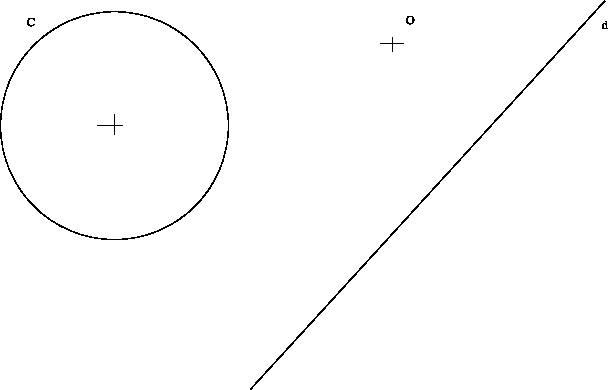
\includegraphics[scale=0.5]{images/img-mour-269-1}

Justifier votre construction.
}
\reponse{
On construit le symétrique $s(d)$ par rapport à $O$ de la droite $d$.
Comme le symétrique de $A$ doit être sur $d$, $A$ doit être sur $s(d)$ et sur le cercle $\mathcal{C}$.

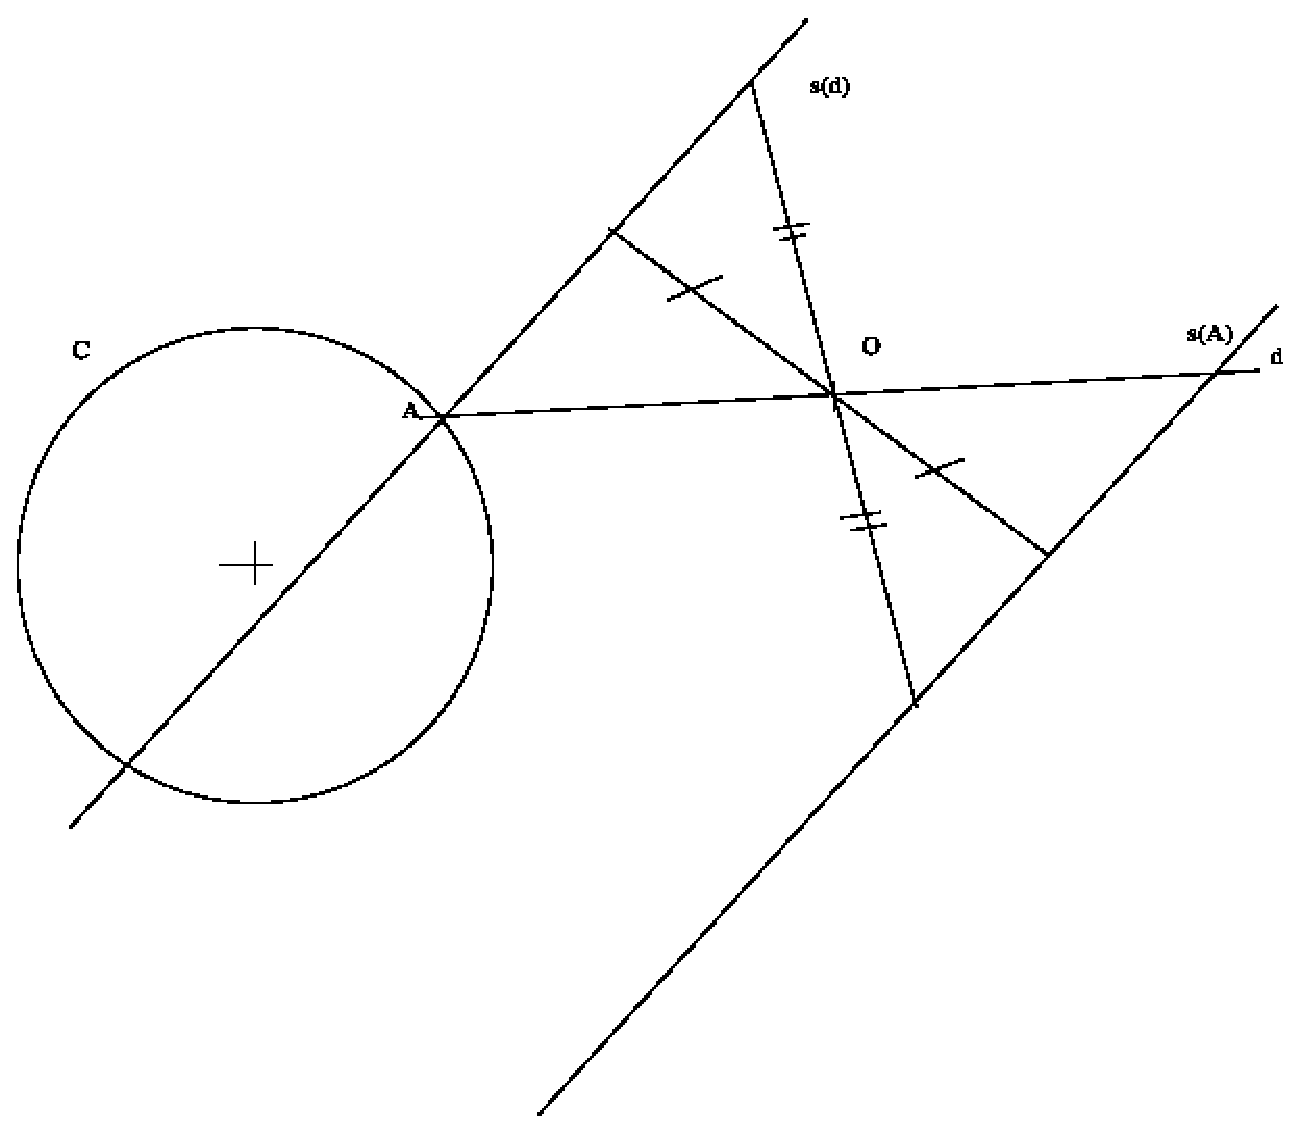
\includegraphics[scale=0.5]{images/img-mour-269-2}
}
}
